\documentclass[a4paper]{article}

\usepackage[T1]{fontenc}
\usepackage{textcomp}
\usepackage{amsmath, amssymb, amsthm}

\usepackage{setspace}
\usepackage{graphicx}
\usepackage{float}

\title{Stats 260 HW: Car Prices}
\date{Oct 05, 2022}
\author{Jack Ruder}


\begin{document}

\doublespacing
\maketitle

\section*{a}
Most likely, price should be transformed. A new car depreciates much faster than an old car, so you would expect the price data to be nonlinear based on age. Also, an old car would bottom out in price, you wouldn't expect to get a car for free just because it is old. However, you cannot log transform values of zero, so we cannot transform age. 

\section*{b}%
\label{sec:b}
\begin{figure}[H]
	\centering
	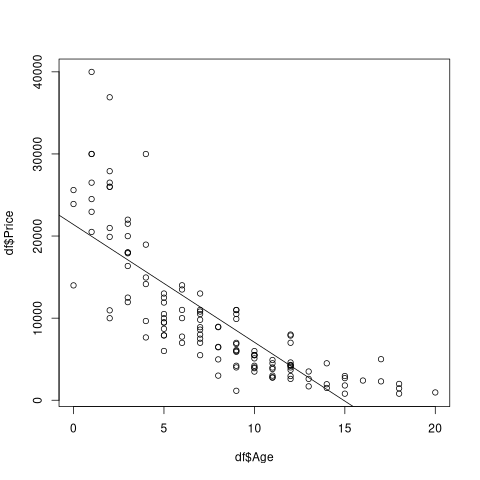
\includegraphics[width=\textwidth]{"../PvA.png"}
\end{figure}
This plot clearly shows that price needs to be transformed, the data is nonlinear concave up. Additionally, we see many datapoints that share the same Age but differ in Price, we should not be able to explain this variation solely off of age.

\section*{c}%
\label{sec:c}
We have,
\begin{equation*}
	\log P = \beta_0 + \beta_1 A,
\end{equation*}
where \(P\) is price, and \(A\) is the age of the car in years. The fitted model is
\begin{equation*}
	\log P = 10.188 -0.165A.
\end{equation*}
These coefficients do not immediately have any intuitive meaning, however we may rewrite this model as 
\begin{equation*}
	P = 26582.3 e^{-0.165A}.
\end{equation*}
This is more telling, we would expect a new car to cost \(26582.3\) dollars. \(-0.165\) is then the rate of decay.

\section*{d}%
\label{sec:d}
\begin{figure}[H]
	\centering
	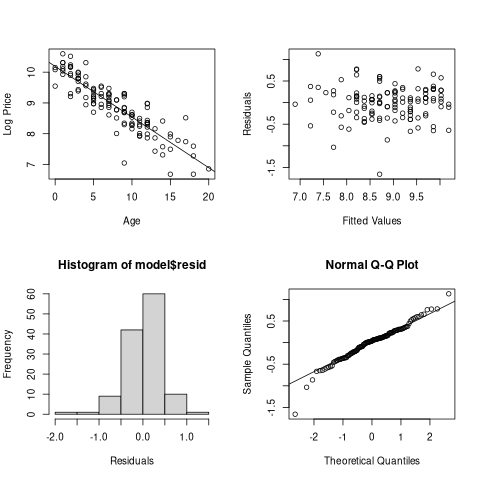
\includegraphics[width=\textwidth]{"../logPvA.png"}
\end{figure}
The residuals in this model prove to be normal. We see the residuals are randomly dispersed around zero, and the Q-Q plot shows very short tails. Looking at the scatterplot for \(\log\) Price vs Age, it seems that there is a potential overfit on the higher leverage ages (>16), but for now the results appear to be quite good.

\section*{e}%
\label{sec:e}
We have an \(R^2\) of \(0.7941\). This is a pretty good explanation of the error in the data, considering how many datapoints have repeated Age values for differing Price values.

\section*{f}%
\label{sec:f}
A t-test on the slope with a value of \(t=-21.69\) yields a \(p\)-value of \(2 \cdot 10^{-16}\), nearly zero. This means Age is an extremely good predictor of \(\log\) Price. That is, given no relation between Price and Age, the probability was nearly zero that we have seen the extreme pattern in the data. The F statistic is much larger than 1, so we see that much of the variation is due to chance. Overall, this model does very well.

\section*{g}%
\label{sec:g}
The upper bound is -0.1496, with a lower bound of -0.1797, with an estimate of -0.165

\section*{h}%
\label{sec:h}
Based on the above analysis, we confidently may say that the price of a Mazda decays with age. The price starts at an estimated 26582 dollars, and exponentially decays at a rate of \(k=-0.165\). There is still a large degree of unexplained variation in price, but a good portion of it is due to chance, or at least unexplainable by any available data to us.

\section*{i}%
\label{sec:i}

We estimate the median car price of a 1985 Mazda was 9893.228. With 95\% probability, we expect that the median price was between 9184.430 and 10656.726.

\section*{j}%
\label{sec:j}

We predict that a new sale of a 1985 Mazda in 1991 would be 9893.228. 95\% of the new sales at that time would have fallen between 4551.881 and 21502.311


\end{document}
